% !TEX root =  ../main_manuscript.tex 
\section{Results}
For patients in the PRIAS dataset, the probability of obtaining reclassification within the first five and ten years is 33\% and 42\%, respectively (see Figure \ref{fig:npmle_plot}). That is, ideally more than 50\% of the patients do not require any biopsy in the first ten years. We next discuss the results from the joint model fitted to the PRIAS dataset. For every ten years increase in a patient age the corresponding adjusted hazard ratio of reclassification is 1.45~(95\%CI:~1.30--1.63). For an increase in fitted $\log_2\{\mbox{PSA + 1}\}$ value from the first quartile of fitted values (2.36) to the third quartile (3.07), the corresponding adjusted hazard ratio of reclassification is 0.99~(95\%CI:~0.89--1.11). On the other hand an increase in fitted $\log_2\{\mbox{PSA + 1}\}$ velocity from the first quartile of fitted velocity (-0.09) to the third quartile (0.31), the corresponding adjusted hazard ratio of reclassification is 2.47~(95\%CI:~1.93--2.99). These results indicate that the velocity of $\log_2\{\mbox{PSA + 1}\}$ measurements is a stronger predictor of hazard of reclassification than the $\log_2\{\mbox{PSA + 1}\}$ value. Detailed parameter estimates are presented in Tables 2, 3 and 5 of Appendix A.4.

Using the joint model fitted to the PRIAS dataset we made risk predictions for GS7 in real PRIAS patients. As shown in Figure 4 of Appendix B, these risk estimates become more accurate as more data is gathered over follow-up. The risk estimates also increase when time last biopsy increases. For these risk predictions we calculated the time dependent area under the receiver operating characteristic curves (AUC) and the root mean squared prediction error (RMSPE). These are shown in Figure~\ref{fig:auc_pe}. For predictions within PRIAS (internal validation), the time-dependent AUC was between 0.62 and 0.69, and RMSPE between 0.23 and 0.37 over the whole follow-up period. For validation in external cohorts, the AUC was similar to the AUC of PRIAS for all cohorts during the first three years of follow-up. The RMPSE however differed much more during the same period. The AS cohorts closest to PRIAS in terms of RMSPE were Johns Hopkins Active Surveillance and Memorial Sloan Kettering Cancer Center Active Surveillance. Detailed AUC and RMSPE results for all cohorts with 95\% bootstrapped confidence intervals are presented in Table 6 to Table 11 of Appendix B.

\begin{figure}
\centerline{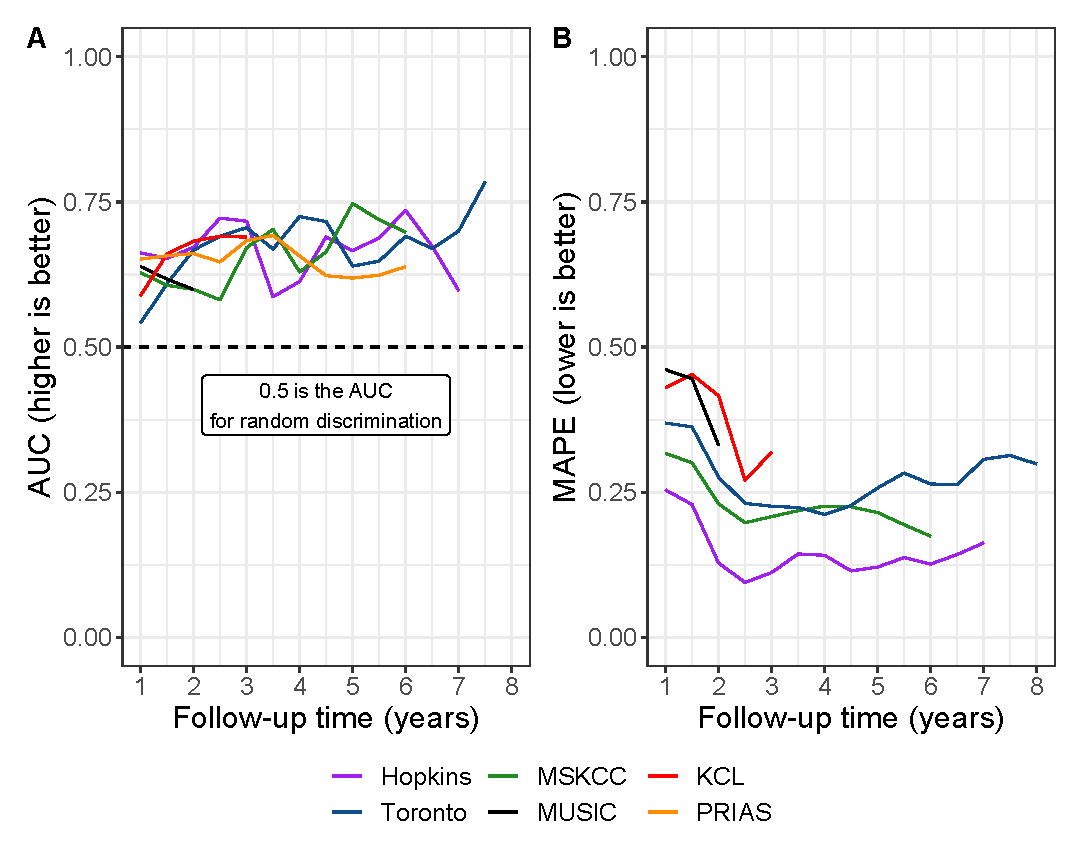
\includegraphics[width=\columnwidth]{images/auc_pe.eps}}
\caption{\textbf{Validation of predictions of Gleason $\geq$ 7 (GS7)}. In \textbf{Panel~A} we can see that the time dependent area under the receiver operating characteristic curve or AUC (measure of discrimination) is above 0.5 in PRIAS (internal validation), and in Toronto, JHAS, MSKCC, KCL, and MUSIC AS cohorts (external validation). In \textbf{Panel~B} we can see that the time dependent root mean squared prediction error or RMSPE (measure of calibration) is similar for PRIAS, and JHAS and Toronto cohorts. The bootstrapped 95\% confidence interval for these estimates are presented in Table 6 to Table 11 of Appendix B. Full names of Cohorts are \textit{PRIAS}: Prostate Cancer International Active Surveillance, \textit{Toronto}: University of Toronto Active Surveillance, \textit{JHAS}: Johns Hopkins Active Surveillance, \textit{MSKCC}: Memorial Sloan Kettering Cancer Center Active Surveillance, \textit{KCL}: King's College London Active Surveillance, \textit{MUSIC}: Michigan Urological Surgery Improvement Collaborative Active Surveillance.}
\label{fig:auc_pe}
\end{figure}

Using the risk predictions for GS7, we developed personalized schedules of biopsy for real PRIAS patients (see Figure \ref{fig:demo_pat1} and Appendix C's Figure 6, 7, 8 and 9). In all of these patients the biopsies denoted by `B' show that personalized schedules schedule fewer biopsies than fixed schedules. At the same time the expected time delay in detection of GS7 is less than an year for personalized schedules. We have implemented this approach in a web-application (\url{www.ourapp.url}) for practical use.